\begin{figure}
\centering

\begin{tikzpicture} %[every node/.style={draw=black}]
% \draw[help lines] (0,0) grid (4,2);
\matrix [row sep=0cm, column sep=0cm, style={align=center}] (my matrix) at (2,1)
{
\node[style={anchor=center}] {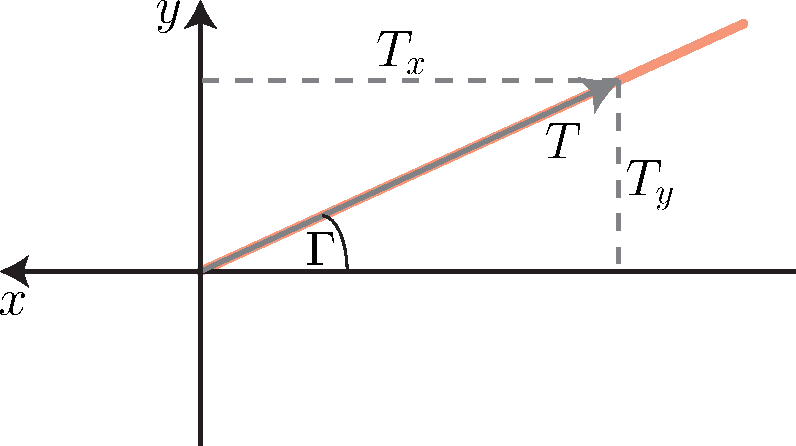
\includegraphics[width=0.42\linewidth]{figures/cableTension.pdf}}; %\fill[blue] (0,0) circle (2pt);
&
\node[style={anchor=center}] {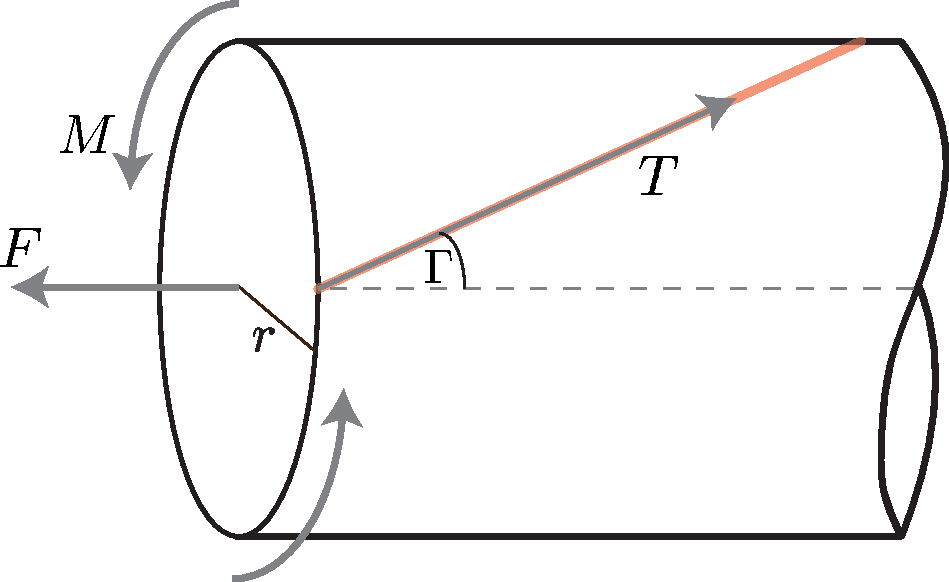
\includegraphics[width=0.42\linewidth]{figures/fiberTension2.pdf}}; %\fill[blue] (0,0) circle (2pt);

\\
\node (a) {(a)}; & \node (c) {(c)};
\\

\begin{axis}[
    xlabel={\footnotesize{$\Gamma$}},
    ylabel={\footnotesize{$T_x/T_y$}},
    ymin=-10, ymax=10, ytick={0}, ylabel near ticks,
    xmin=0, xmax=90, xtick={0,90}, xticklabel=$\pgfmathprintnumber{\tick}^\circ$, xlabel near ticks,
    tick label style={font=\footnotesize},
    width=0.5\linewidth,
    anchor=center,
]
    \addplot [domain=0:90, dashed] {0};
    \addplot [domain=1:90, samples=100] {-cot(x)};
\end{axis};
& 
\begin{axis}[
    xlabel={\footnotesize{$\Gamma$}},
    ylabel={\footnotesize{$F/M$}},
    ymin=-10, ymax=10, ytick={0}, ylabel near ticks,
    xmin=0, xmax=90, xtick={0,54.7,90}, xticklabel=$\pgfmathprintnumber{\tick}^\circ$, xlabel near ticks,
    tick label style={font=\footnotesize},
    width=0.5\linewidth,
    anchor=center,
]
    \addplot [domain=0:90, dashed] {0};
    \addplot [domain=1:90, samples=100] {(1-2*cot(x)^2) / (2*cot(x))};
    \addplot [mark=none, dashed] coordinates {(54.7,-10) (54.7,10)};
\end{axis};
%\fill[blue] (0,0) circle (2pt);

\\
\node (b) {(b)}; & \node (d) {(d)};
\\
};
\end{tikzpicture}

\caption{By changing the fiber angle of a FREE, it can be configured to produce a large range of force/torque combinations. To understand this, we consider how (a) the angle at which a fiber is pulled in a plane affects (b) the ratio between the $x$ and $y$ components of the pulling force. Similarly, by (c) wrapping the plane into a cylinder and accounting for an internal pressure force pushing out on the endcap, the (d) ratio between axial force and twisting moment can be arbitrarily set by changing the fiber angle.}
\label{fig:FMratios}
\end{figure}